% UTF-8。保留原文文字、颜色、字号、缩进和空段落；最后一项参数是可编辑文本。

% 原文段落 109；2 需求分析
\newpage
\begin{WordParagraph}{center}{18}{\WordAutoLine{18}{1.25}}{0}{0}{0}{7.8}{7.8}
\WordAutoSpaceOn
\WordRun{Times}{Hei}{18}{1}{0}{000000}{0}{2}%
\WordRun{Hei}{Hei}{18}{1}{0}{000000}{0}{\WordSpace{1}}%
\WordRun{Times}{Hei}{18}{1}{0}{000000}{0}{需求分析}
\end{WordParagraph}

% 原文段落 110；（黑体小2加粗居中,字母、阿拉伯数字为Time New Roman小2号加粗）
\begin{WordParagraph}{center}{12}{\WordAutoLine{12}{1.25}}{0}{0}{0}{7.8}{7.8}
\WordAutoSpaceOn
\WordRun{Kai}{Kai}{12}{0}{0}{FF0000}{0}{（黑体小2加粗居中}%
\WordRun{Kai}{Kai}{12}{0}{0}{FF0000}{0}{,字母、阿拉伯数字为Time\WordSpace{1}New\WordSpace{1}Roman小2号加粗}%
\WordRun{Kai}{Kai}{12}{0}{0}{FF0000}{0}{）}
\end{WordParagraph}

% 原文段落 111；2.1 需求分析概述（黑体4号加粗,字母、阿拉伯数字为Time New Roman4号加粗）
\begin{WordParagraph}{both}{14}{\WordAutoLine{14}{1.25}}{0}{0}{0}{7.8}{7.8}
\WordAutoSpaceOn
\WordRun{Times}{Song}{14}{1}{0}{000000}{0}{2.1}%
\WordRun{Hei}{Hei}{14}{1}{0}{000000}{0}{\WordSpace{1}需求分析概述}%
\WordRun{Kai}{Kai}{12}{0}{0}{FF0000}{0}{（黑体4号加粗,字母、阿拉伯数字为Time\WordSpace{1}New\WordSpace{1}Roman4号加粗）}
\end{WordParagraph}

% 原文段落 112；选取合适的图表准确说明用户需求，明确所做系统要实现的目标。表的格式示例如下：
\begin{WordParagraph}{both}{12}{\WordAutoLine{12}{1.5}}{0}{0}{24}{0}{0}
\WordAutoSpaceOn
\WordRun{Song}{Song}{12}{0}{0}{000000}{0}{选取合适的图表准确说明用户需求，明确所做系统要实现的目标。表的格式示例如下：}
\end{WordParagraph}

% 原文段落 113；表2-1□××××××××××
\begin{WordParagraph}{center}{12}{15}{0}{0}{24}{0}{0}
\WordAutoSpaceOn
\WordRun{Hei}{Hei}{12}{0}{0}{000000}{0}{表}%
\WordRun{Times}{Hei}{12}{0}{0}{000000}{0}{2-1}%
\WordRun{Hei}{Hei}{12}{0}{0}{000000}{0}{□\WordHAnsi{Hei}{×}\hskip0pt plus .05em\relax{}\WordHAnsi{Hei}{×}\hskip0pt plus .05em\relax{}\WordHAnsi{Hei}{×}\hskip0pt plus .05em\relax{}\WordHAnsi{Hei}{×}\hskip0pt plus .05em\relax{}\WordHAnsi{Hei}{×}\hskip0pt plus .05em\relax{}\WordHAnsi{Hei}{×}\hskip0pt plus .05em\relax{}\WordHAnsi{Hei}{×}\hskip0pt plus .05em\relax{}\WordHAnsi{Hei}{×}\hskip0pt plus .05em\relax{}\WordHAnsi{Hei}{×}\hskip0pt plus .05em\relax{}\WordHAnsi{Hei}{×}\hskip0pt plus .05em\relax{}}
\end{WordParagraph}

% 原文段落 114；
\begin{WordParagraph}{center}{12}{15}{0}{0}{24}{0}{0}
\WordAutoSpaceOn
\WordEmpty
\end{WordParagraph}

% 原文表格：宽396pt、左缩进14.4pt、列宽72/108/108/108pt。
\par\begingroup
\WordLatinSong\CJKfamily{WordSong}\fontsize{12bp}{15bp}\selectfont
\setlength{\tabcolsep}{0pt}
\renewcommand{\arraystretch}{1}
\setlength{\extrarowheight}{0pt}
\setlength{\arrayrulewidth}{.5bp}
\noindent\hspace*{14.4bp}\begin{tabular}{@{}>{\centering\arraybackslash}m{72bp}@{}*{3}{>{\centering\arraybackslash}m{108bp}@{}}}
\specialrule{1.5bp}{0pt}{0pt}
\WordRun{Song}{Song}{12}{0}{0}{000000}{0}{\WordHAnsi{Song}{×}\hskip0pt plus .05em\relax{}\WordHAnsi{Song}{×}\hskip0pt plus .05em\relax{}\WordHAnsi{Song}{×}\hskip0pt plus .05em\relax{}\WordHAnsi{Song}{×}\hskip0pt plus .05em\relax{}\WordHAnsi{Song}{×}\hskip0pt plus .05em\relax{}} & \WordRun{Song}{Song}{12}{0}{0}{000000}{0}{\WordHAnsi{Song}{×}\hskip0pt plus .05em\relax{}\WordHAnsi{Song}{×}\hskip0pt plus .05em\relax{}\WordHAnsi{Song}{×}\hskip0pt plus .05em\relax{}} & \WordRun{Song}{Song}{12}{0}{0}{000000}{0}{\WordHAnsi{Song}{×}\hskip0pt plus .05em\relax{}\WordHAnsi{Song}{×}\hskip0pt plus .05em\relax{}\WordHAnsi{Song}{×}\hskip0pt plus .05em\relax{}} & \WordRun{Song}{Song}{12}{0}{0}{000000}{0}{\WordHAnsi{Song}{×}\hskip0pt plus .05em\relax{}\WordHAnsi{Song}{×}\hskip0pt plus .05em\relax{}\WordHAnsi{Song}{×}\hskip0pt plus .05em\relax{}} \\
\specialrule{.5bp}{0pt}{0pt}
\WordRun{Song}{Song}{12}{0}{0}{000000}{0}{\WordHAnsi{Song}{×}\hskip0pt plus .05em\relax{}\WordHAnsi{Song}{×}\hskip0pt plus .05em\relax{}\WordHAnsi{Song}{×}\hskip0pt plus .05em\relax{}\WordHAnsi{Song}{×}\hskip0pt plus .05em\relax{}\WordHAnsi{Song}{×}\hskip0pt plus .05em\relax{}} & \WordRun{Song}{Song}{12}{0}{0}{000000}{0}{\WordHAnsi{Song}{×}\hskip0pt plus .05em\relax{}\WordHAnsi{Song}{×}\hskip0pt plus .05em\relax{}} & \WordRun{Song}{Song}{12}{0}{0}{000000}{0}{\WordHAnsi{Song}{×}\hskip0pt plus .05em\relax{}\WordHAnsi{Song}{×}\hskip0pt plus .05em\relax{}} & \WordRun{Song}{Song}{12}{0}{0}{000000}{0}{\WordHAnsi{Song}{×}\hskip0pt plus .05em\relax{}\WordHAnsi{Song}{×}\hskip0pt plus .05em\relax{}} \\
\WordRun{Song}{Song}{12}{0}{0}{000000}{0}{\WordHAnsi{Song}{×}\hskip0pt plus .05em\relax{}\WordHAnsi{Song}{×}\hskip0pt plus .05em\relax{}\WordHAnsi{Song}{×}\hskip0pt plus .05em\relax{}\WordHAnsi{Song}{×}\hskip0pt plus .05em\relax{}\WordHAnsi{Song}{×}\hskip0pt plus .05em\relax{}} & \WordRun{Song}{Song}{12}{0}{0}{000000}{0}{\WordHAnsi{Song}{×}\hskip0pt plus .05em\relax{}\WordHAnsi{Song}{×}\hskip0pt plus .05em\relax{}} & \WordRun{Song}{Song}{12}{0}{0}{000000}{0}{\WordHAnsi{Song}{×}\hskip0pt plus .05em\relax{}\WordHAnsi{Song}{×}\hskip0pt plus .05em\relax{}} & \WordRun{Song}{Song}{12}{0}{0}{000000}{0}{\WordHAnsi{Song}{×}\hskip0pt plus .05em\relax{}\WordHAnsi{Song}{×}\hskip0pt plus .05em\relax{}} \\
\WordRun{Song}{Song}{12}{0}{0}{000000}{0}{\WordHAnsi{Song}{×}\hskip0pt plus .05em\relax{}\WordHAnsi{Song}{×}\hskip0pt plus .05em\relax{}\WordHAnsi{Song}{×}\hskip0pt plus .05em\relax{}\WordHAnsi{Song}{×}\hskip0pt plus .05em\relax{}\WordHAnsi{Song}{×}\hskip0pt plus .05em\relax{}} & \WordRun{Song}{Song}{12}{0}{0}{000000}{0}{\WordHAnsi{Song}{×}\hskip0pt plus .05em\relax{}\WordHAnsi{Song}{×}\hskip0pt plus .05em\relax{}} & \WordRun{Song}{Song}{12}{0}{0}{000000}{0}{\WordHAnsi{Song}{×}\hskip0pt plus .05em\relax{}\WordHAnsi{Song}{×}\hskip0pt plus .05em\relax{}} & \WordRun{Song}{Song}{12}{0}{0}{000000}{0}{\WordHAnsi{Song}{×}\hskip0pt plus .05em\relax{}\WordHAnsi{Song}{×}\hskip0pt plus .05em\relax{}} \\
\cline{2-4}
\WordRun{Song}{Song}{12}{0}{0}{000000}{0}{\WordHAnsi{Song}{×}\hskip0pt plus .05em\relax{}\WordHAnsi{Song}{×}\hskip0pt plus .05em\relax{}\WordHAnsi{Song}{×}\hskip0pt plus .05em\relax{}\WordHAnsi{Song}{×}\hskip0pt plus .05em\relax{}\WordHAnsi{Song}{×}\hskip0pt plus .05em\relax{}} & \WordRun{Song}{Song}{12}{0}{0}{000000}{0}{\WordHAnsi{Song}{×}\hskip0pt plus .05em\relax{}\WordHAnsi{Song}{×}\hskip0pt plus .05em\relax{}} & \WordRun{Song}{Song}{12}{0}{0}{000000}{0}{\WordHAnsi{Song}{×}\hskip0pt plus .05em\relax{}\WordHAnsi{Song}{×}\hskip0pt plus .05em\relax{}} & \WordRun{Song}{Song}{12}{0}{0}{000000}{0}{\WordHAnsi{Song}{×}\hskip0pt plus .05em\relax{}\WordHAnsi{Song}{×}\hskip0pt plus .05em\relax{}} \\
\specialrule{1.5bp}{0pt}{0pt}
\end{tabular}
\par\endgroup

% 原文段落 116；
\begin{WordParagraph}{both}{12}{15}{0}{0}{24}{0}{0}
\WordAutoSpaceOn
\WordEmpty
\end{WordParagraph}

% 原文段落 117；（表标题：位于表格上方，黑体小4号，字母、阿拉伯数字为Time New Roman小4号，表内容：宋体5号，字母、阿拉伯数字为Time New Roman 5号）
\begin{WordParagraph}{both}{12}{15}{0}{0}{24}{0}{0}
\WordAutoSpaceOn
\WordRun{Kai}{Kai}{12}{0}{0}{FF0000}{0}{（表标题：位于表格上方，黑体小4号，字母、阿拉伯数字为Time\WordSpace{1}New\WordSpace{1}Roman小4号，表内容：宋体5号，字母、阿拉伯数字为Time\WordSpace{1}New\WordSpace{1}Roman\WordSpace{1}5号）}
\end{WordParagraph}

% 原文段落 118；
\begin{WordParagraph}{left}{12}{\WordAutoLine{12}{1.5}}{6.85}{0}{18}{0}{0}
\WordAutoSpaceOn
\WordEmpty
\end{WordParagraph}

% 原文段落 119；××××××××××××××××××××××××××× (如图2-1所示)，图的格式示例如下：
\begin{WordParagraph}{left}{12}{\WordAutoLine{12}{1.5}}{6.85}{0}{18}{0}{0}
\WordAutoSpaceOn
\WordRun{Song}{Song}{12}{0}{0}{000000}{0}{\WordHAnsi{Song}{×}\hskip0pt plus .05em\relax{}\WordHAnsi{Song}{×}\hskip0pt plus .05em\relax{}\WordHAnsi{Song}{×}\hskip0pt plus .05em\relax{}\WordHAnsi{Song}{×}\hskip0pt plus .05em\relax{}\WordHAnsi{Song}{×}\hskip0pt plus .05em\relax{}\WordHAnsi{Song}{×}\hskip0pt plus .05em\relax{}\WordHAnsi{Song}{×}\hskip0pt plus .05em\relax{}\WordHAnsi{Song}{×}\hskip0pt plus .05em\relax{}\WordHAnsi{Song}{×}\hskip0pt plus .05em\relax{}\WordHAnsi{Song}{×}\hskip0pt plus .05em\relax{}\WordHAnsi{Song}{×}\hskip0pt plus .05em\relax{}\WordHAnsi{Song}{×}\hskip0pt plus .05em\relax{}\WordHAnsi{Song}{×}\hskip0pt plus .05em\relax{}\WordHAnsi{Song}{×}\hskip0pt plus .05em\relax{}\WordHAnsi{Song}{×}\hskip0pt plus .05em\relax{}\WordHAnsi{Song}{×}\hskip0pt plus .05em\relax{}\WordHAnsi{Song}{×}\hskip0pt plus .05em\relax{}\WordHAnsi{Song}{×}\hskip0pt plus .05em\relax{}\WordHAnsi{Song}{×}\hskip0pt plus .05em\relax{}\WordHAnsi{Song}{×}\hskip0pt plus .05em\relax{}\WordHAnsi{Song}{×}\hskip0pt plus .05em\relax{}\WordHAnsi{Song}{×}\hskip0pt plus .05em\relax{}\WordHAnsi{Song}{×}\hskip0pt plus .05em\relax{}\WordHAnsi{Song}{×}\hskip0pt plus .05em\relax{}\WordHAnsi{Song}{×}\hskip0pt plus .05em\relax{}\WordHAnsi{Song}{×}\hskip0pt plus .05em\relax{}\WordHAnsi{Song}{×}\hskip0pt plus .05em\relax{}\WordSpace{1}}%
\WordRun{Times}{Song}{12}{0}{0}{000000}{0}{(如图2-1所示)，图的格式示例如下：}
\end{WordParagraph}

% 原文段落 120；
\begin{WordParagraph}{center}{12}{\WordAutoLine{12}{1.5}}{6}{0}{-6}{0}{0}
\WordAutoSpaceOn
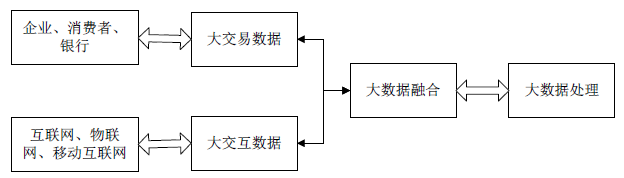
\includegraphics[width=14.0758cm,height=3.9688cm]{assets/diagram.png}
\end{WordParagraph}

% 原文段落 121；图2-1□××××××××××
\begin{WordParagraph}{center}{12}{\WordAutoLine{12}{1.5}}{6}{0}{-6}{0}{0}
\WordAutoSpaceOn
\WordRun{Hei}{Hei}{12}{0}{0}{000000}{0}{图}%
\WordRun{Times}{Song}{12}{0}{0}{000000}{0}{2-1}%
\WordRun{Hei}{Hei}{12}{0}{0}{000000}{0}{□\WordHAnsi{Hei}{×}\hskip0pt plus .05em\relax{}\WordHAnsi{Hei}{×}\hskip0pt plus .05em\relax{}\WordHAnsi{Hei}{×}\hskip0pt plus .05em\relax{}\WordHAnsi{Hei}{×}\hskip0pt plus .05em\relax{}\WordHAnsi{Hei}{×}\hskip0pt plus .05em\relax{}\WordHAnsi{Hei}{×}\hskip0pt plus .05em\relax{}\WordHAnsi{Hei}{×}\hskip0pt plus .05em\relax{}\WordHAnsi{Hei}{×}\hskip0pt plus .05em\relax{}\WordHAnsi{Hei}{×}\hskip0pt plus .05em\relax{}\WordHAnsi{Hei}{×}\hskip0pt plus .05em\relax{}}
\end{WordParagraph}

% 原文段落 122；（图标题：位于图下方，黑体小4号，字母、阿拉伯数字为Time New Roman小4号）
\begin{WordParagraph}{both}{12}{15}{0}{0}{24}{0}{0}
\WordAutoSpaceOn
\WordRun{Kai}{Kai}{12}{0}{0}{FF0000}{0}{（图标题：位于图下方，黑体小4号，字母、阿拉伯数字为Time\WordSpace{1}New\WordSpace{1}Roman小4号）}
\end{WordParagraph}

% 原文段落 123；
\begin{WordParagraph}{both}{12}{\WordAutoLine{12}{1.5}}{0}{0}{24}{0}{0}
\WordAutoSpaceOn
\WordEmpty
\end{WordParagraph}

% 原文段落 124；2.2 UML相关需求分析图（黑体4号加粗,字母、阿拉伯数字为Time New Roman4号加粗）
\begin{WordParagraph}{both}{14}{\WordAutoLine{14}{1.25}}{0}{0}{0}{7.8}{7.8}
\WordAutoSpaceOn
\WordRun{Times}{Song}{14}{1}{0}{000000}{0}{2.2}%
\WordRun{Hei}{Hei}{14}{1}{0}{000000}{0}{\WordSpace{1}UML相关需求分析图}%
\WordRun{Kai}{Kai}{12}{0}{0}{FF0000}{0}{（黑体4号加粗,字母、阿拉伯数字为Time\WordSpace{1}New\WordSpace{1}Roman4号加粗）}
\end{WordParagraph}

% 原文段落 125；选取合适的图表准确说明用户需求，明确所做系统要实现的目标。
\begin{WordParagraph}{both}{12}{\WordAutoLine{12}{1.5}}{0}{0}{24}{0}{0}
\WordAutoSpaceOn
\WordRun{Song}{Song}{12}{0}{0}{000000}{0}{选取合适的图表准确说明用户需求，明确所做系统要实现的目标。}
\end{WordParagraph}

% 原文段落 126；
\begin{WordParagraph}{both}{12}{\WordAutoLine{12}{1.5}}{0}{0}{0}{0}{0}
\WordAutoSpaceOn
\WordEmpty
\end{WordParagraph}

\begin{samepage}

% 原文段落 127；2.3 原型系统设计（黑体4号加粗,字母、阿拉伯数字为Time New Roman4号加粗）
\begin{WordParagraph}{both}{14}{\WordAutoLine{14}{1.25}}{0}{0}{0}{7.8}{7.8}
\WordAutoSpaceOn
\WordRun{Times}{Song}{14}{1}{0}{000000}{0}{2.3}%
\WordRun{Hei}{Hei}{14}{1}{0}{000000}{0}{\WordSpace{1}原型系统设计}%
\WordRun{Kai}{Kai}{12}{0}{0}{FF0000}{0}{（黑体4号加粗,字母、阿拉伯数字为Time\WordSpace{1}New\WordSpace{1}Roman4号加粗）}
\end{WordParagraph}

% 原文段落 128；运用工具设计原型系统，从而更准确说明主要功能和用户交互界面。
\begin{WordParagraph}{both}{12}{\WordAutoLine{12}{1.5}}{0}{0}{24}{0}{0}
\WordAutoSpaceOn
\WordRun{Song}{Song}{12}{0}{0}{000000}{0}{运用工具设计原型系统，从而更准确说明主要功能和用户交互界面。}
\end{WordParagraph}

% 原文段落 129；
\begin{WordParagraph}{both}{12}{\WordAutoLine{12}{1.5}}{0}{0}{0}{0}{0}
\WordAutoSpaceOn
\WordEmpty
\end{WordParagraph}

% 原文段落 130；.......
\begin{WordParagraph}{center}{12}{\WordAutoLine{12}{1.5}}{6}{0}{-6}{0}{0}
\WordAutoSpaceOn
\WordRun{Song}{Song}{12}{0}{0}{000000}{0}{.......}
\end{WordParagraph}

% 原文段落 131；--------章与章之间插入分页符----------
\begin{WordParagraph}{center}{12}{\WordAutoLine{12}{1.5}}{0}{0}{0}{0}{0}
\WordAutoSpaceOn
\WordRun{Times}{Song}{12}{0}{0}{000000}{0}{--------章与章之间插入分页符----------}
\end{WordParagraph}

\end{samepage}

% 原文段落 132；
\newpage
\begin{WordParagraph}{left}{12}{\WordAutoLine{12}{1}}{0}{0}{0}{0}{0}
\WordAutoSpaceOn
\WordEmpty
\end{WordParagraph}
